\begin{figure}%
	\centering%
	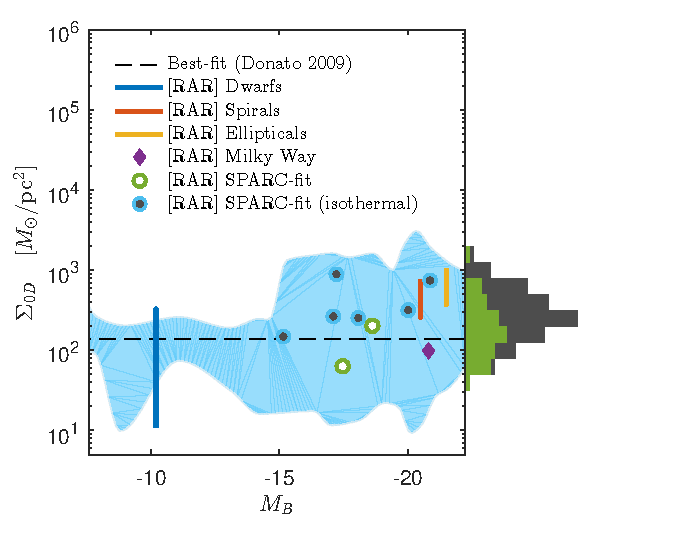
\includegraphics[width=\hsize]{\ROOTPATH/fig.pdf}%
	\caption{Radial acceleration correlation in the Milky Way galaxy. Results from the RAR model (solid line) are compared with McGaugh's empirical fit (dashed line) and NFW model (dot-dashed line). The dotted line describes where the centripetal acceleration of dark and baryonic matter are equal. Thus, in the top-left corner is the dark matter dominated region and in the bottom-right corner is the baryonic matter dominated region. The transition appears at about $\SI{2E-11}{\metre/\second^2}$. In the very high acceleration regime the RAR model predicts an increase of dark matter acceleration due to the degenerate dark matter core in the Galactic center.}%
\label{fig:mw-ac}
\end{figure}